\begin{frame}\frametitle{Why Kalman?}
\begin{columns}[t]
\column{.49\textwidth}
\textbf{I. Blending the measurements}\\ %\begin{block}{}
\vspace{-1em}
\begin{center}
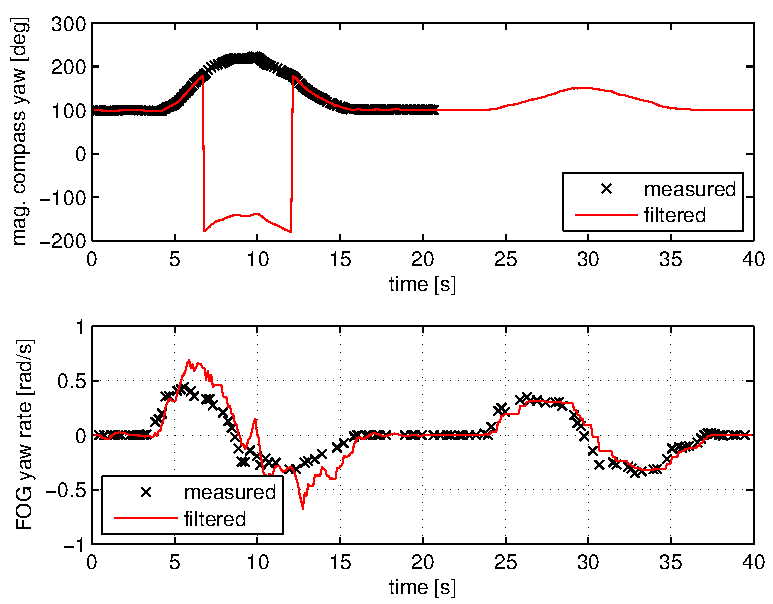
\includegraphics[width=0.8\linewidth]{fig/lostCompass.pdf}
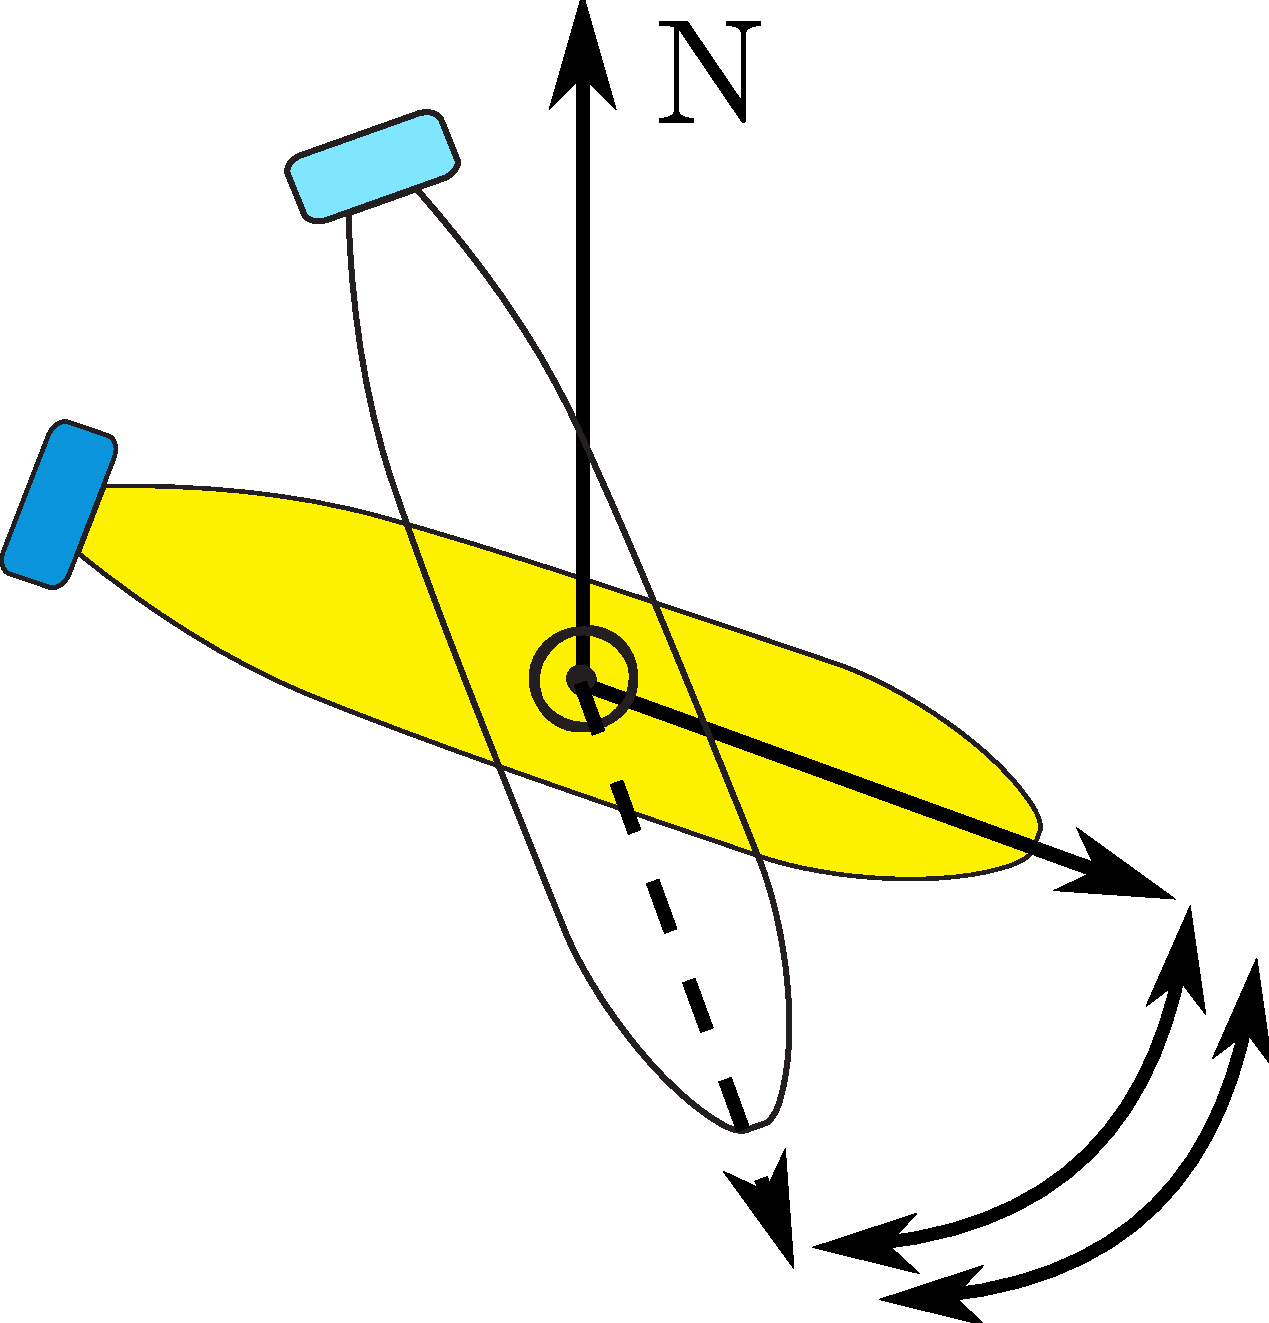
\includegraphics[width=0.19\linewidth]{fig/rotate.pdf} \\
\end{center}
\vspace{-1em}
yaw $(\psi)$ is inferred from compass \& FOG.\\
\textit{EKF benefit}: \pro if one of them stops working - the other one tries to compensate the failure

			\column{.49\textwidth}%$\Rightarrow$ 
			\textbf{II. Prediction \& Filtering} \\ %\begin{block}{}
			If the measurement temporarily fails, EKF keeps predicting. Noisy velocity information is filtered. \\%, with increased uncertainty. \\
			\centering
			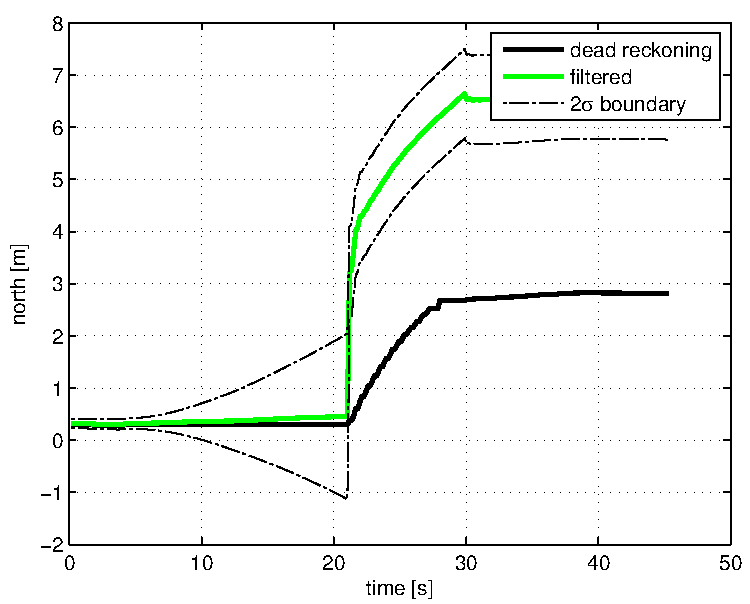
\includegraphics[width=0.49\linewidth]{fig/northLengthPool.pdf} 
			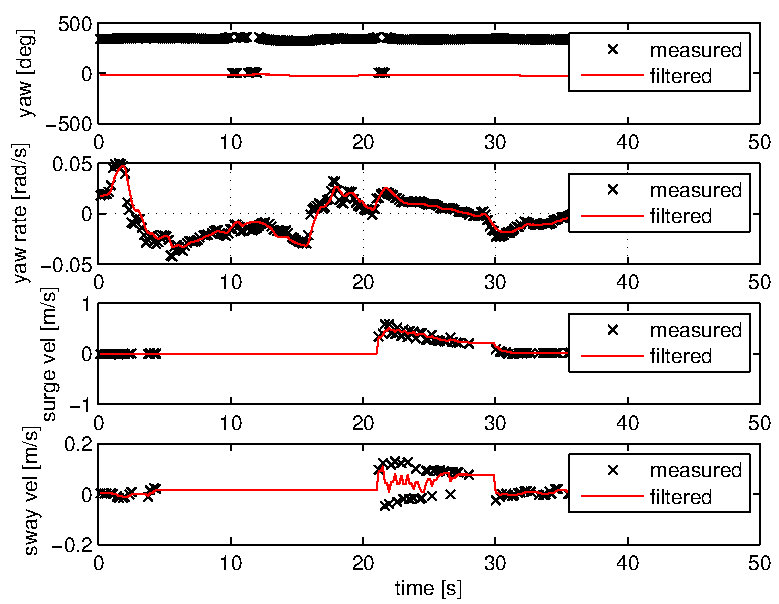
\includegraphics[width=0.49\linewidth]{fig/dynLengthPool.pdf}\\
			\textit{Outcome}: \pro less drift \\
			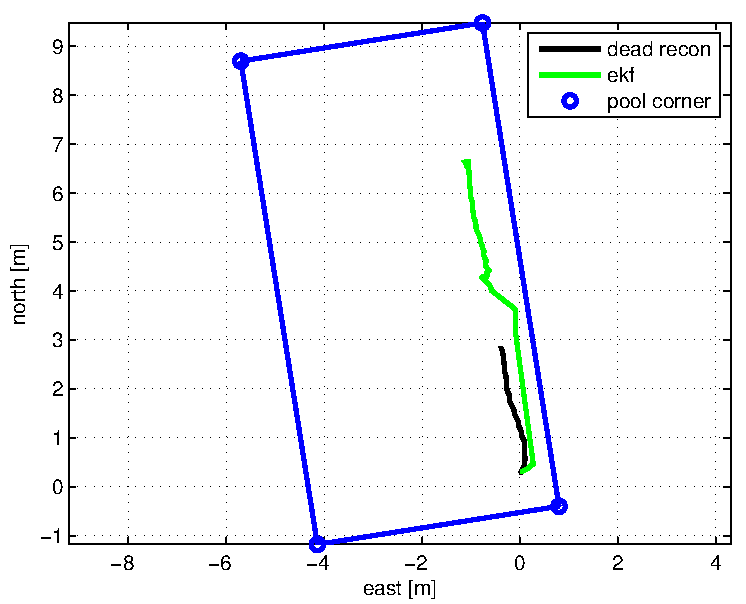
\includegraphics[width=0.5\linewidth]{fig/lengthPool.pdf}  \hspace{0.5em} 
			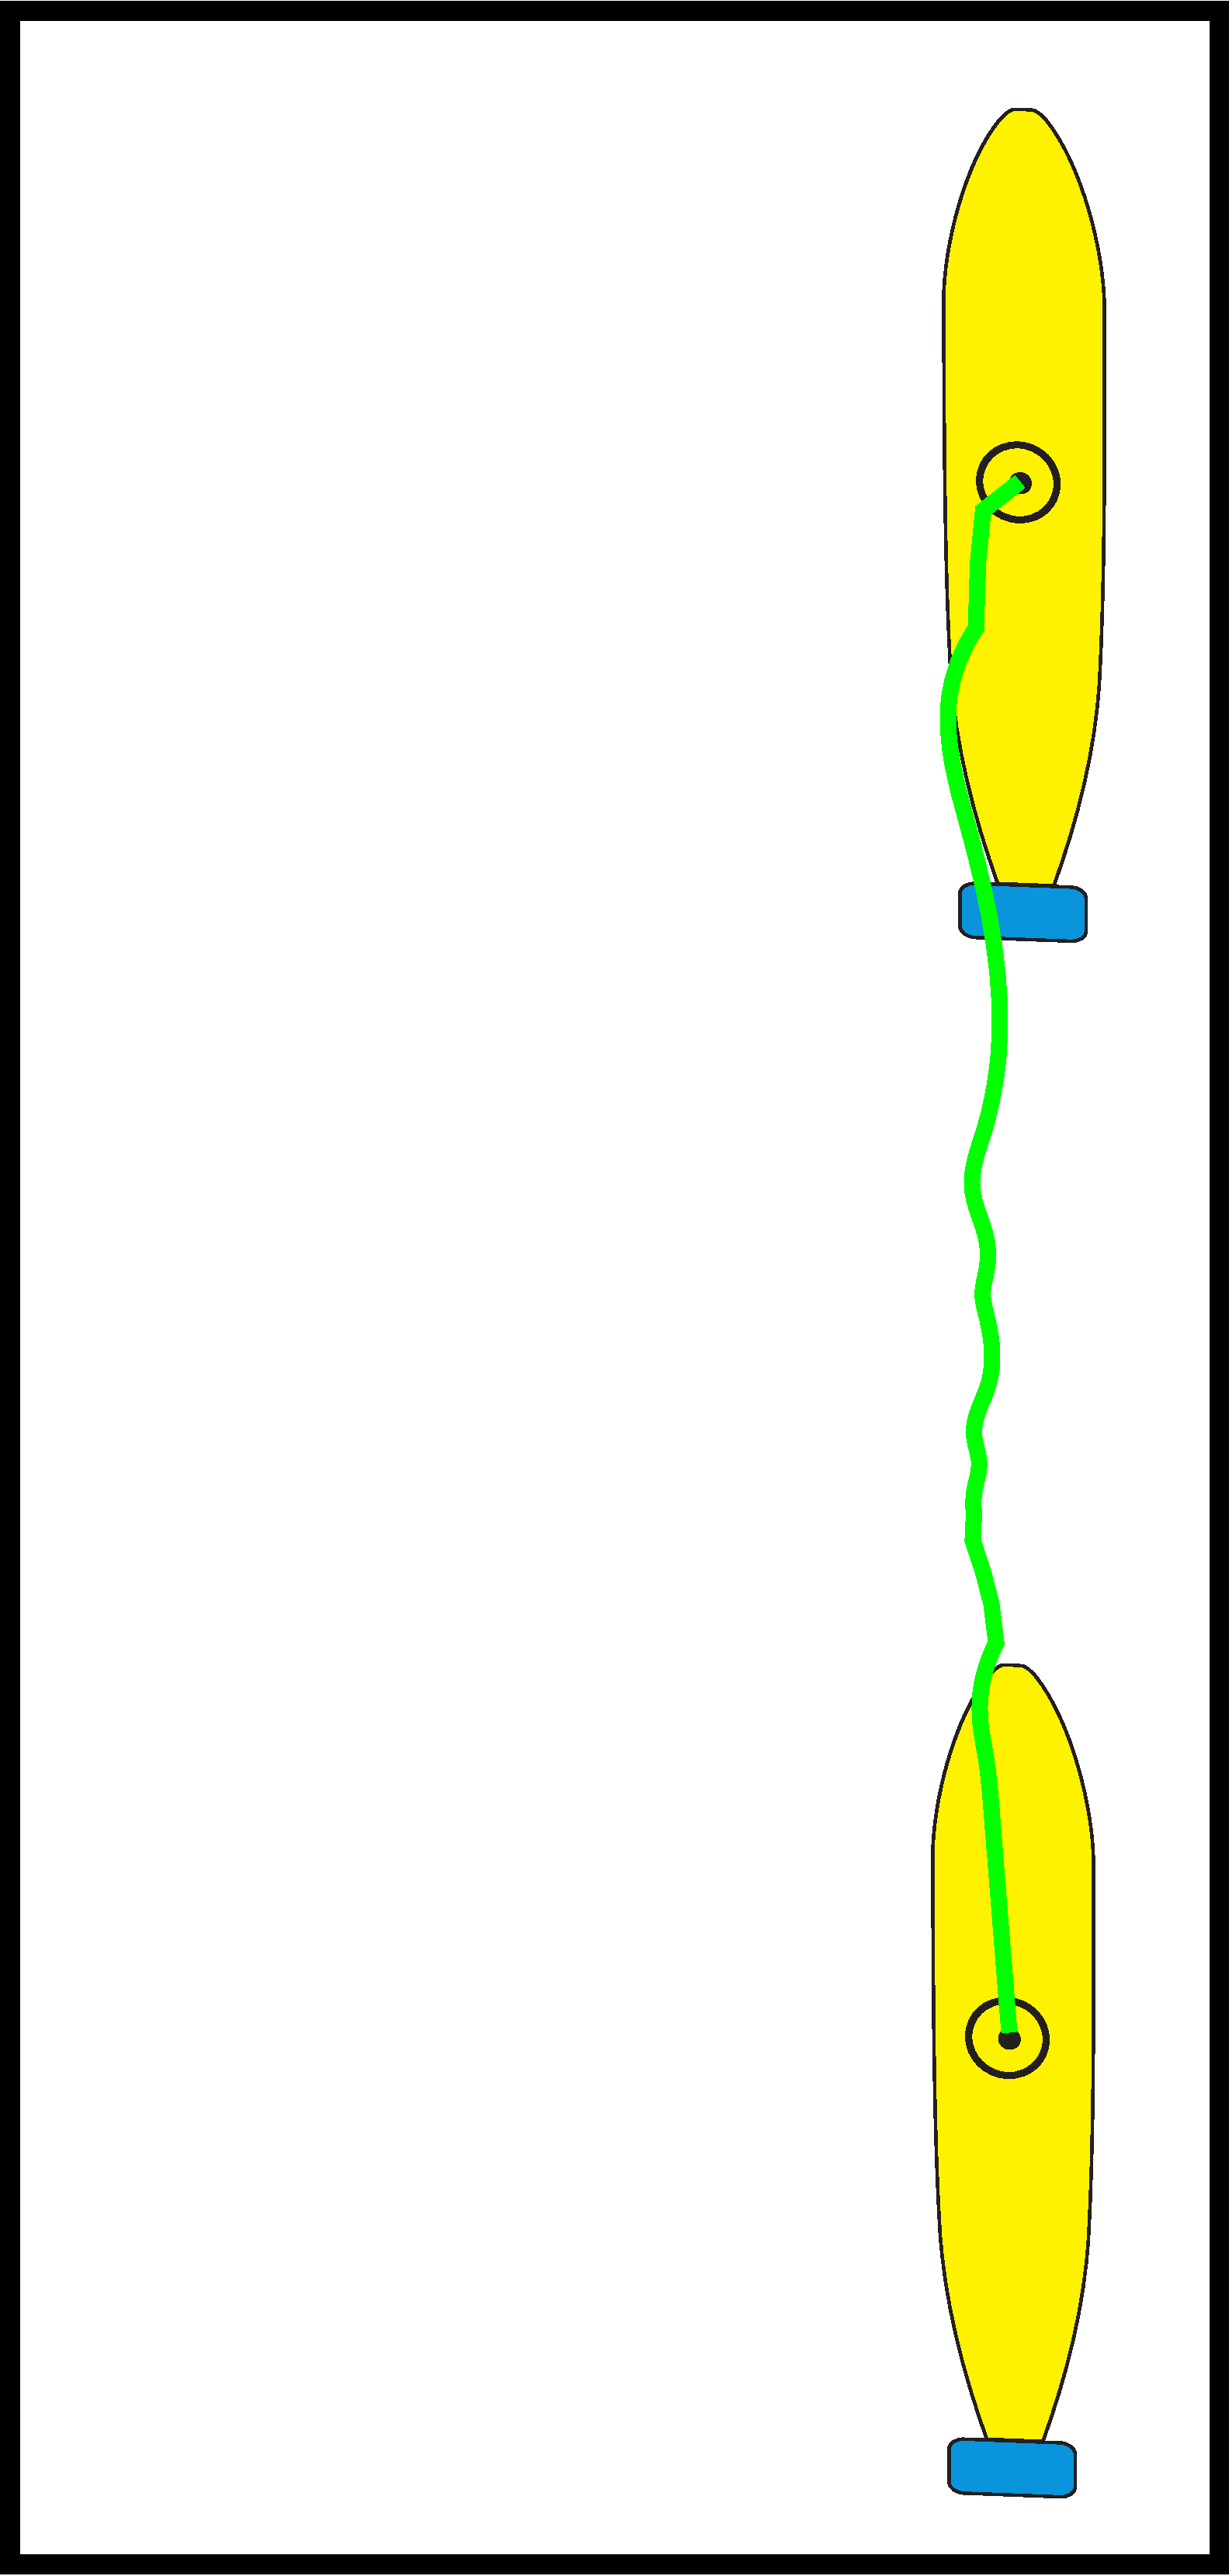
\includegraphics[width=0.15\linewidth]{fig/path.pdf} 
\end{columns}
\textbf{III. Parametric Estimation: }
setting the values of model and observation noise covariance matrices dozes the ``trust'' in model/measurements. 
\end{frame}